\documentclass[12pt]{article}
\usepackage[margin=1in]{geometry}
\usepackage{setspace}
\onehalfspacing

% Start of preamble
%==========================================================================================%
% Required to support mathematical unicode
\usepackage[warnunknown, fasterrors, mathletters]{ucs}
\usepackage[utf8x]{inputenc}

\usepackage[dvipsnames,table,xcdraw]{xcolor}

% Standard mathematical typesetting packages
\usepackage{amsmath,amssymb,amscd,amsthm,amsxtra}
\usepackage{mathtools,mathrsfs,xparse,newtxtext,newtxmath}

% Symbol and utility packages
\usepackage{cancel, textcomp}
\usepackage[mathscr]{euscript}
\usepackage[nointegrals]{wasysym}
\usepackage{apacite}

% Extras
\usepackage{physics}  
\usepackage{tikz-cd} 
\usepackage{microtype}
\usepackage{enumitem}
\usepackage{titling}
\usepackage{graphicx}

% Common shortcuts
\def\mbb#1{\mathbb{#1}}
\def\mfk#1{\mathfrak{#1}}

\def\bN{\mbb{N}}
\def \C{\mbb{C}}
\def \R{\mbb{R}}
\def\bQ{\mbb{Q}}
\def\bZ{\mbb{Z}}
\def \cph{\varphi}
\renewcommand{\th}{\theta}
\def \ve{\varepsilon}
\newcommand{\mg}[1]{\| #1 \|}

% Often helpful macros
\newcommand{\floor}[1]{\left\lfloor#1\right\rfloor}
\newcommand{\ceil}[1]{\left\lceil#1\right\rceil}
\renewcommand{\qed}{\hfill\qedsymbol}
\renewcommand{\P}{\mathbb P\qty}
\newcommand{\E}{\mathbb{E}\qty}
\newcommand{\Cov}{\mathrm{Cov}\qty}
\newcommand{\Var}{\mathrm{Var}\qty}

% Sets
\usepackage{braket}

\graphicspath{{/}}
\usepackage{float}

\newcommand{\SET}[1]{\Set{\mskip-\medmuskip #1 \mskip-\medmuskip}}

% End of preamble
%==========================================================================================%

% Start of commands specific to this file
%==========================================================================================%

\usepackage{listings}  % For lstlisting environment
\usepackage{xcolor}    % For syntax highlighting (optional)

\lstset{
  basicstyle=\ttfamily\small,  % Monospace font, small size
  breaklines=true,             % Enable automatic line breaking
  breakatwhitespace=true,      % Break lines at spaces
  frame=single,                % Add a box around the listing
  columns=fullflexible,        % Allow flexible character spacing
}

%==========================================================================================%
% End of commands specific to this file

\title{CSE 422 HW6}
\date{\today}
\author{Rohan Mukherjee}

\begin{document}
    \maketitle
    \subsection*{Problem 1: Graph Laplacians}
    \begin{enumerate}[leftmargin=\labelsep, label=(\alph*)]
        \item Cycle Laplacian:
        \begin{align*}
            &\begin{bmatrix}
            2 & -1 & 0 & 0 & 0 & 0 & -1 \\
            -1 & 2 & -1 & 0 & 0 & 0 & 0 \\
            0 & -1 & 2 & -1 & 0 & 0 & 0 \\
            0 & 0 & -1 & 2 & -1 & 0 & 0 \\
            0 & 0 & 0 & -1 & 2 & -1 & 0 \\
            0 & 0 & 0 & 0 & -1 & 2 & -1 \\
            -1 & 0 & 0 & 0 & 0 & -1 & 2
            \end{bmatrix} \\[1em]
        \end{align*}
        Spoke and Wheel Laplacian:
        \begin{align*}
            &\begin{bmatrix}
            3 & -1 & 0 & 0 & 0 & -1 & -1 \\
            -1 & 3 & -1 & 0 & 0 & 0 & -1 \\
            0 & -1 & 3 & -1 & 0 & 0 & -1 \\
            0 & 0 & -1 & 3 & -1 & 0 & -1 \\
            0 & 0 & 0 & -1 & 3 & -1 & -1 \\
            -1 & 0 & 0 & 0 & -1 & 3 & -1 \\
            -1 & -1 & -1 & -1 & -1 & -1 & 6
            \end{bmatrix} \\[1em]
        \end{align*}
        Line Graph Laplacian:
        \begin{align*}
            &\begin{bmatrix}
            1 & -1 & 0 & 0 & 0 & 0 & 0 \\
            -1 & 2 & -1 & 0 & 0 & 0 & 0 \\
            0 & -1 & 2 & -1 & 0 & 0 & 0 \\
            0 & 0 & -1 & 2 & -1 & 0 & 0 \\
            0 & 0 & 0 & -1 & 2 & -1 & 0 \\
            0 & 0 & 0 & 0 & -1 & 2 & -1 \\
            0 & 0 & 0 & 0 & 0 & -1 & 1
            \end{bmatrix} \\[1em]
        \end{align*}
        Line Point Laplacian:
        \begin{align*}
            &\begin{bmatrix}
            2 & -1 & 0 & 0 & 0 & 0 & -1 \\
            -1 & 3 & -1 & 0 & 0 & 0 & -1 \\
            0 & -1 & 3 & -1 & 0 & 0 & -1 \\
            0 & 0 & -1 & 3 & -1 & 0 & -1 \\
            0 & 0 & 0 & -1 & 3 & -1 & -1 \\
            0 & 0 & 0 & 0 & -1 & 2 & -1 \\
            -1 & -1 & -1 & -1 & -1 & -1 & 6
            \end{bmatrix}
        \end{align*}        
        \item Here is the picture for the cycle Laplacian:
        \begin{figure}[H]
            \centering
            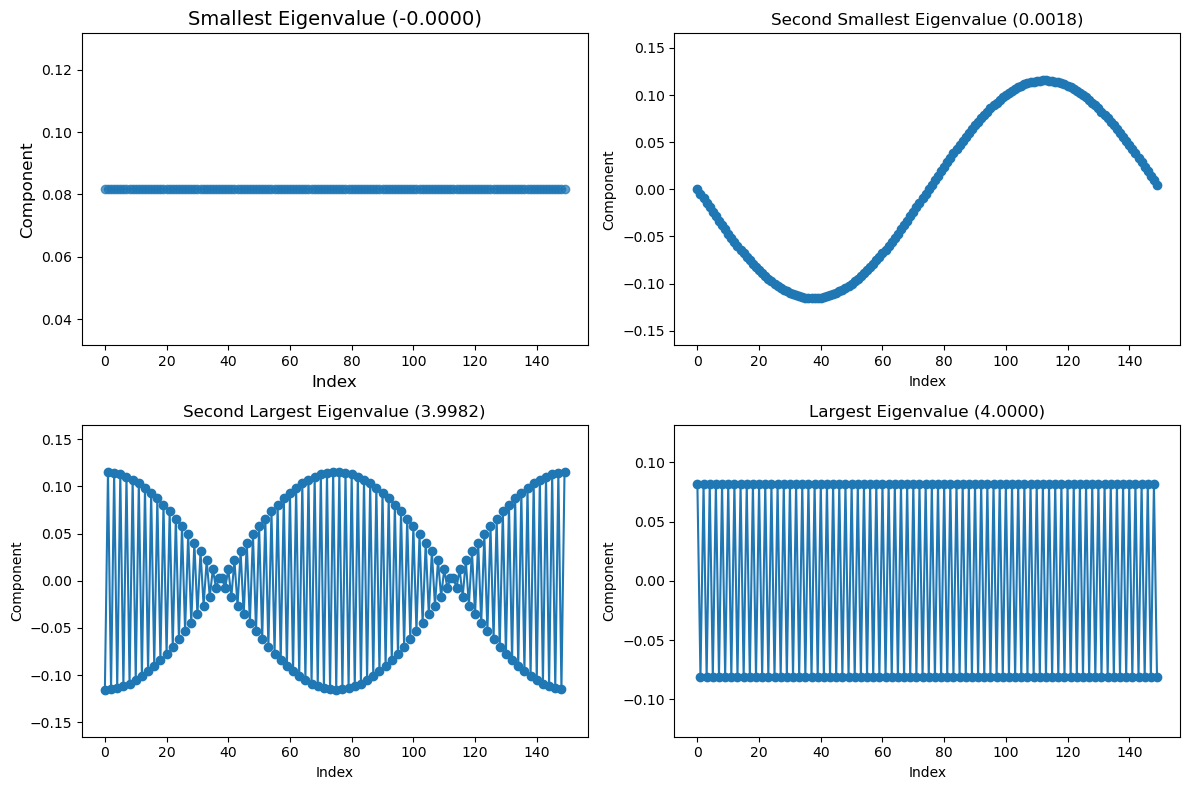
\includegraphics[width=0.8\textwidth]{cycle_L.png}
            \caption{Cycle Laplacian}
        \end{figure}
        And cycle adjacency matrix:
        \begin{figure}[H]
            \centering
            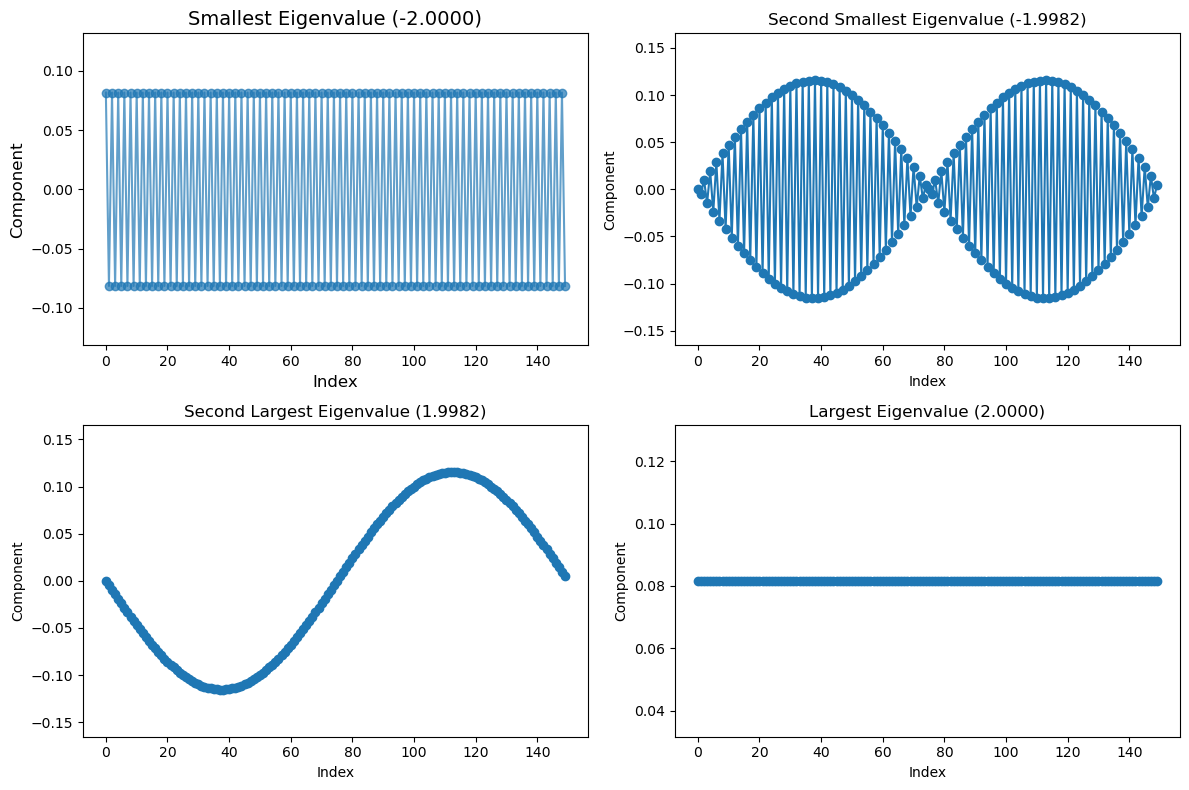
\includegraphics[width=0.8\textwidth]{cycle_A.png}
            \caption{Cycle Adjacency List}
        \end{figure}
        
        Spoke and wheel laplacian:
        \begin{figure}[H]
            \centering
            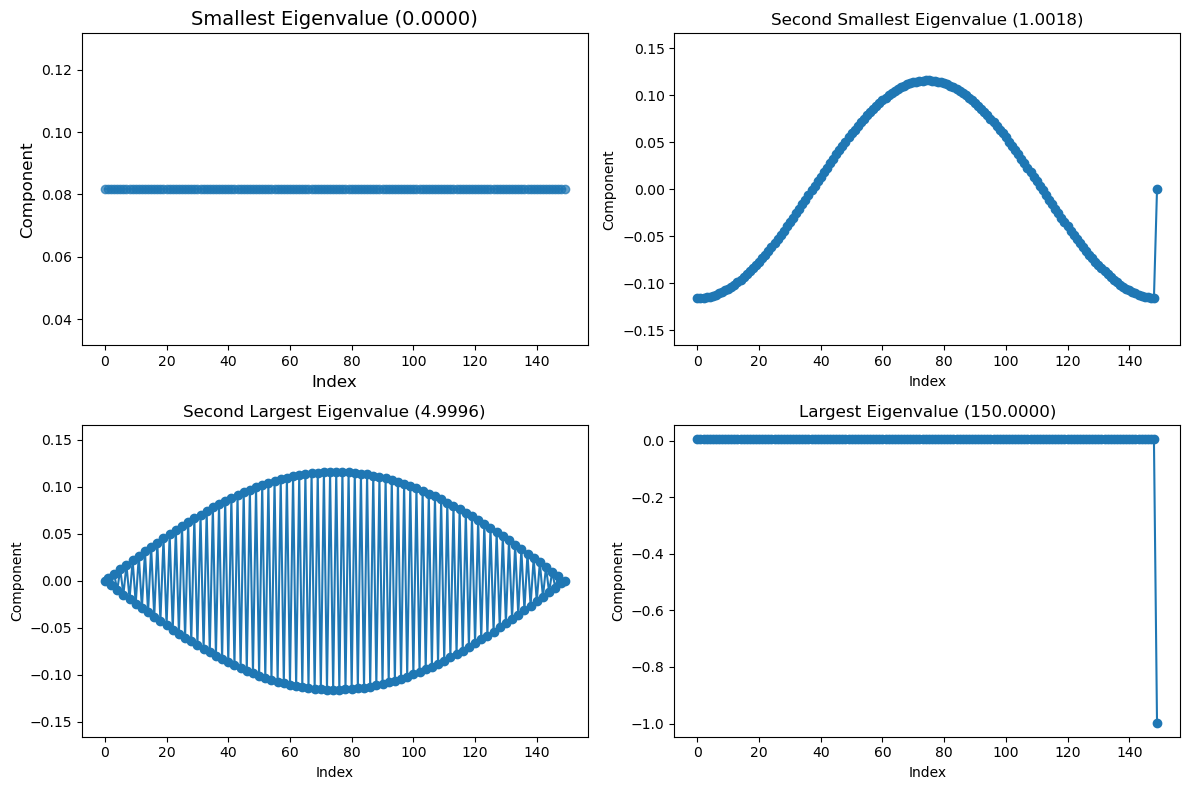
\includegraphics[width=0.8\textwidth]{spoke_L.png}
            \caption{Spoke and Wheel Laplacian}
        \end{figure}
        And spoke and wheel adjacency matrix:
        \begin{figure}[H]
            \centering
            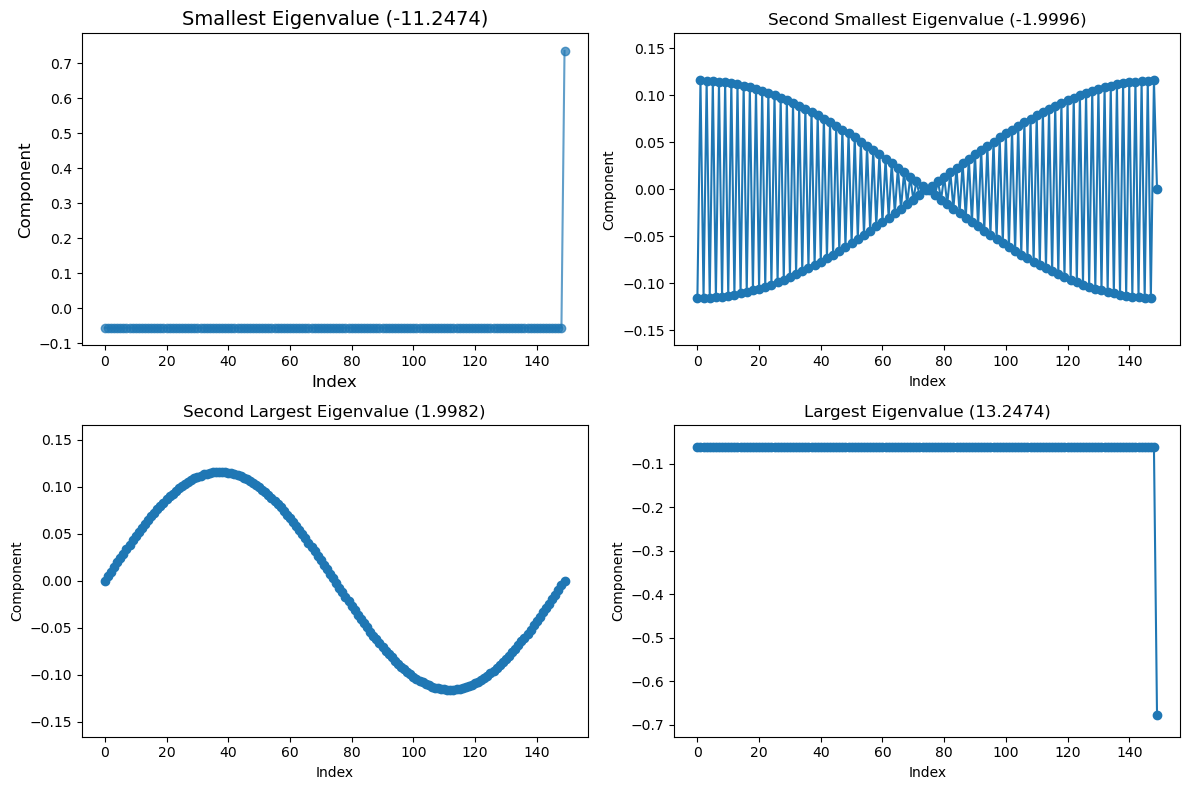
\includegraphics[width=0.8\textwidth]{spoke_A.png}
            \caption{Spoke and Wheel Adjacency List}
        \end{figure}
        Line graph laplacian:
        \begin{figure}[H]
            \centering
            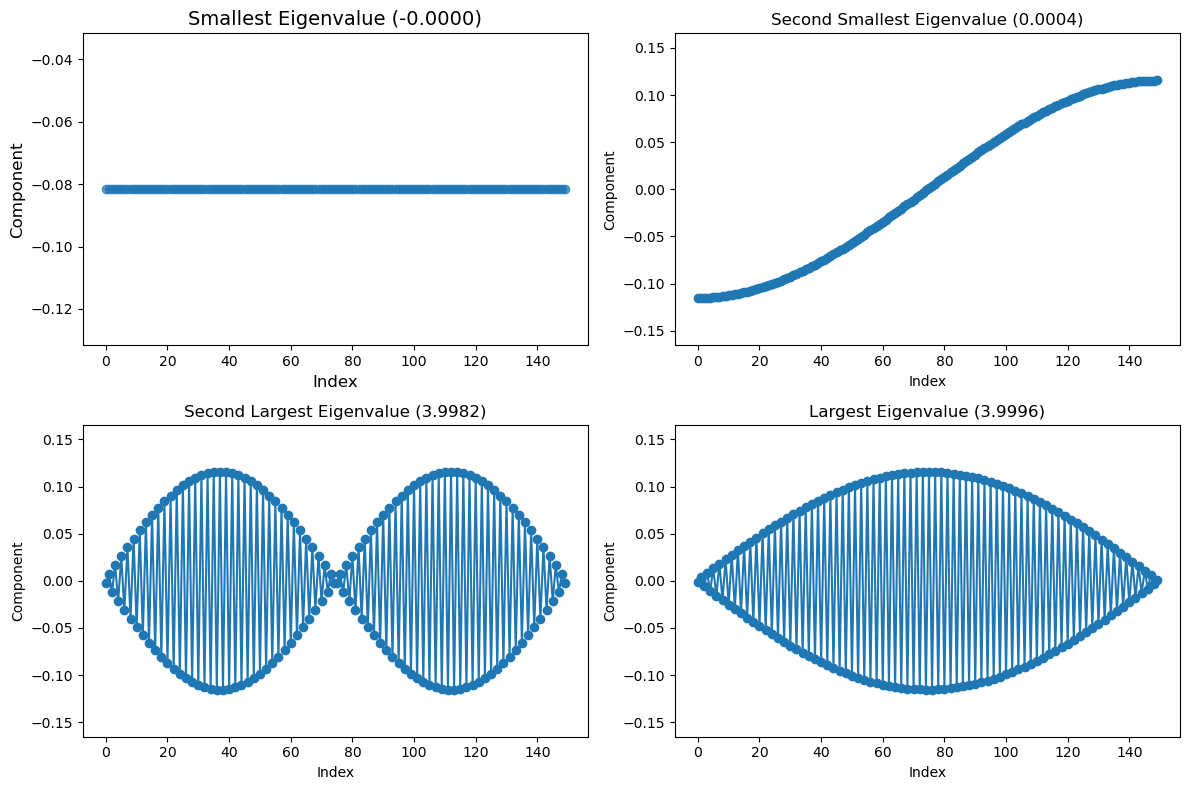
\includegraphics[width=0.8\textwidth]{line_L.png}
            \caption{Line Graph Laplacian}
        \end{figure}
        And line graph adjacency matrix:
        \begin{figure}[H]
            \centering
            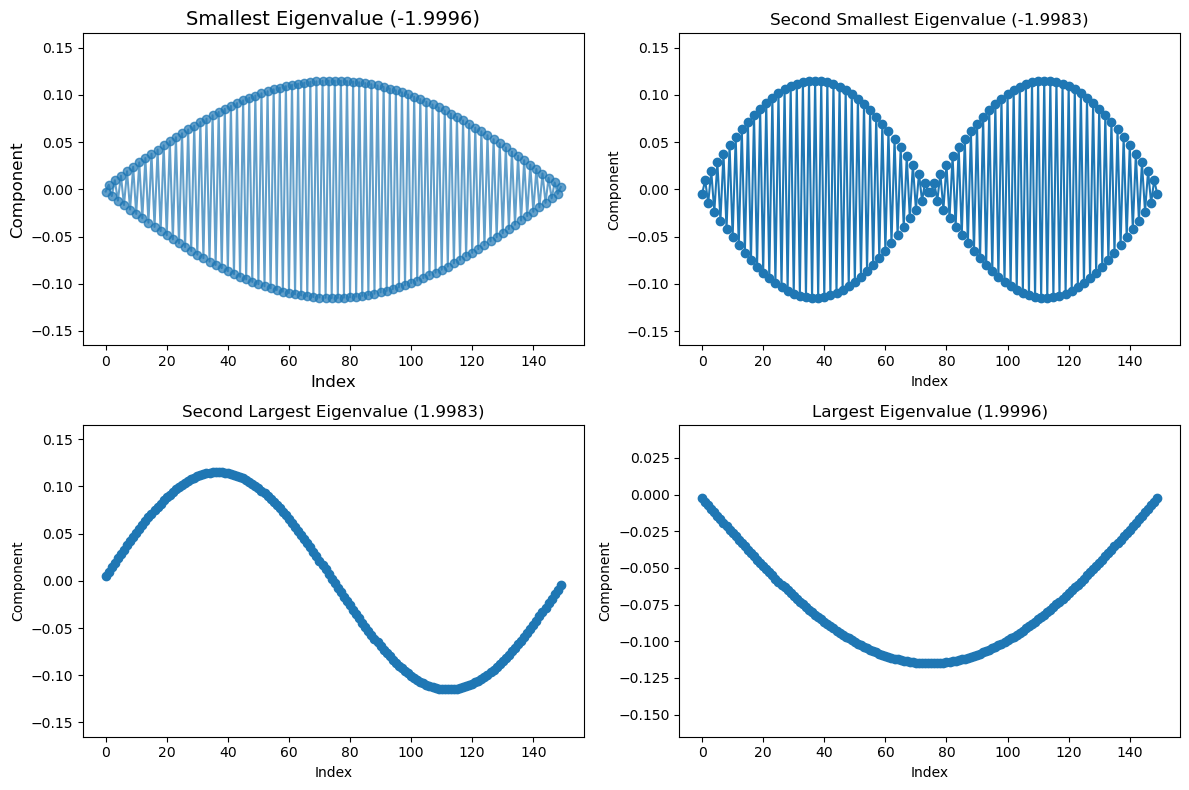
\includegraphics[width=0.8\textwidth]{line_A.png}
            \caption{Line Graph Adjacency List}
        \end{figure}
        Line point laplacian:
        \begin{figure}[H]
            \centering
            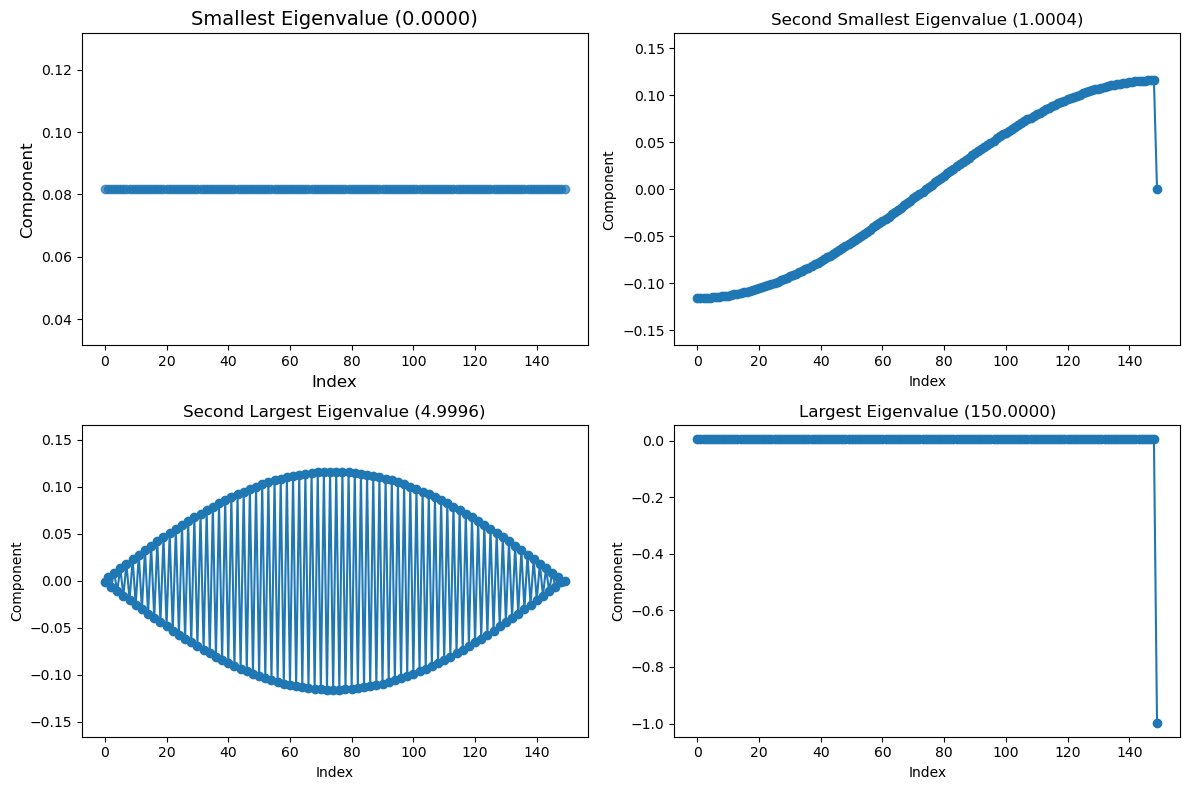
\includegraphics[width=0.8\textwidth]{line_point_L.png}
            \caption{Line Point Laplacian}
        \end{figure}
        And line point adjacency matrix:
        \begin{figure}[H]
            \centering
            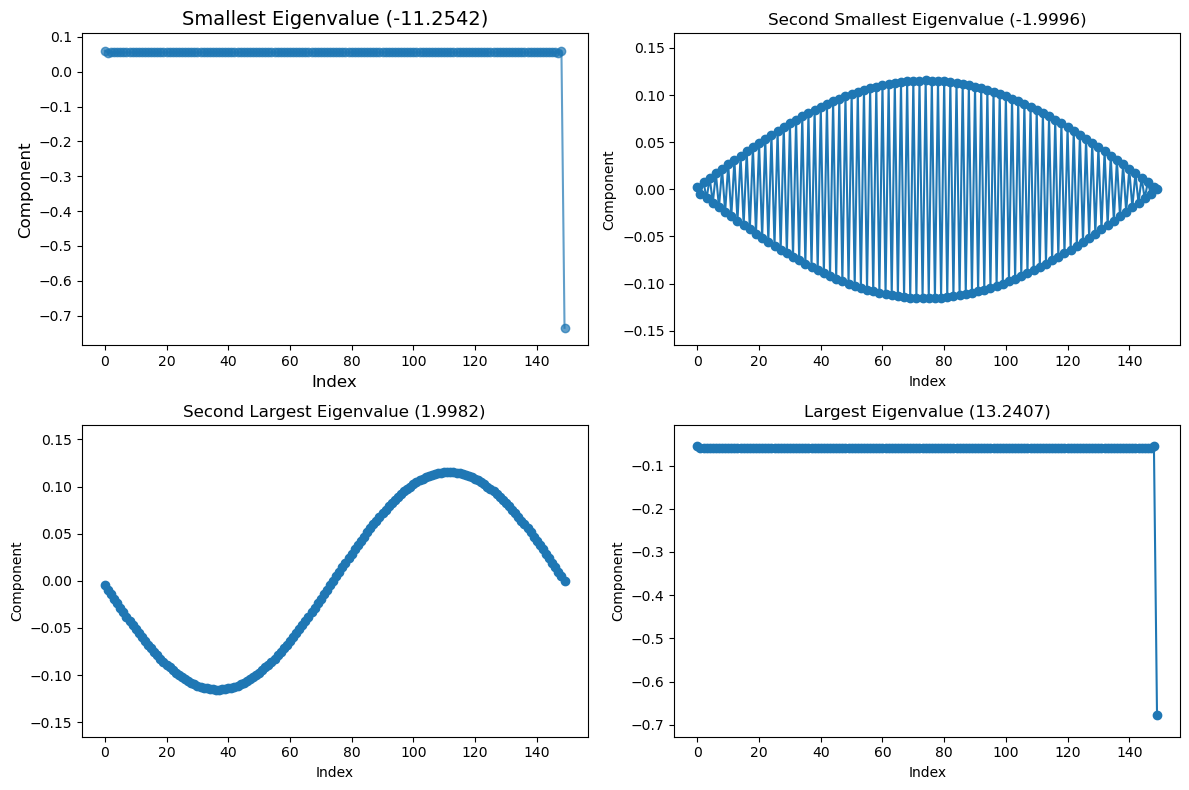
\includegraphics[width=0.8\textwidth]{line_point_A.png}
            \caption{Line Point Adjacency List}
        \end{figure}

        \item The difference between the largest and second largest eigenvalue is called the spectral gap, and it is a measure of how connected a graph is. In the pictures, you can see that the line graph and cycle graph have very small spectral gap. On the other hand, the spoke and wheel graph and line + a point graph have huge gaps. This is because I would consider the line graph with a point and spoke and wheel graph much more connected than the other two. In the cycle, there are many points that are $n/2$ away from each other, and in the line, most points are more than $n/2$ from each other, going all the way up to $n-1$. On the other hand, the distance between any two vertices in spoke and wheel is at most 2, and in the line graph with a point its also only 2. So, these graphs are much more connected, and hence have a much larger spectral gap.

        \item 
        Throughout this, we use for the Laplacian graph, 
        \begin{align*}
            x^T L_G x = \sum_{i \sim j} (x_i-x_i)^2
        \end{align*}
        To be small, you want neighbors to be close together. So small eigenvectors should give good clusterings. On the flip side, to be large you want neighbors to have vastly different values. This interpretation of neighbors being far from each other is similar to coloring, or vertex propulsion. 

        For the cycle graph Laplacian, you would suspect all the graphs to be invariant over cyclic permutations of the indices. That's why you get these oscillations. The largest eigenvector, which wants to repel neighbors, is able to do so perfectly by assigning each neighbor a different color (I suspect this would look different if we had an odd cycle). The second largest eigenvector does relatively the same thing but has to look slightly different as it is orthogonal to the first. The smallest eigenvector is of course the all 1s vector, and the second smallest eigenvector, which represents clusters, oscillates up and down. You would want close neighbors to be close, and ones that are far to be far. However, it increases up to a point, and then because you can wrap around, the distances start actually getting smaller, which is why it goes back down. Notice the contrast with the line graph below.

        For the spoke and wheel graph Laplacian, the second smallest eigenvector is symbolic of clustering. For this graph, every vertex is at most distance 2 away from each other. So you would naturally want The points that are 1 away from each other in the same cluster. Then just by the nature of the graph you would want those that are 2 away to be a fit further. Putting this together, you get an increase then a gradual decrease. Since the graph is a cycle, you would expect it to end and start at around the same point. Finally, as below, the last node is connected to everything else, so it can go in any cluster, so in expectation it outputs 0. The largest eigenvector is clear, to maximize the energy, or separate neighbors most effectively, you would have all the outer nodes in one cluster and the center in its own. But if you want something orthogonal to this, you would necessarily need something that oscillates like on the second smallest eigenvector, which this time it assigns neighbors different colors. The smallest eigenvector is again the all 1s vector.

        For the line graph Laplacian, the smallest eigenvector is the all 1s. The second smallest eigenvector, symbolic of clustering, gradually increases over time. This is related to how the line graph looks. You would want close things to be in the same cluster, but far away points to be far away. This is why the first and last point have the largest gap. Following this intuition, you would get a gradual increase. The largest eigenvector is related to neighbors repelling. This would be a 2-coloring, and indeed since the line is perfectly 2 colorable, that is what you get here. I believe you get an up to down picture in this case, which is different from the cycle, because the first and last node have smaller degree, so you would want to give them lower weight. Putting this together, you would get a picture that goes up and then back down. The second largest eigenvector is symbolic of repelling too, but must be orthogonal to the first. Since this one really can be 2-colored, you get almost the same picture but with double the frequency as to make it orthogonal.

        For the line and point Laplacian, like before the smallest eigenvector of the laplacian graph is the all 1s vector. The second smallest eigenvector gives a good clustering. In this case, it gives a very similar graph to the line graph. However, the 150th point has a value of 0. I believe this happens because the last point, being connected to everything, could go into any clustering equally, so it just gets confused and outputs 0 (or it would be 0 in expectation). This is also my favorite explanation for why $a \in \R^3$ has $a \times a = 0$, there are infinitely many vectors perpendicular to $a$, so it gets confused and just outputs 0. The largest eigenvector is symbolic of a coloring, where neighbors repel themselves. Indeed, with the last point connected to everything, every other point would want to repel the last point, so that's why its off on its own while the rest are together. The second largest eigenvector captures repelling too, but an orthogonal direction to the first, which is why it gives an alternating structure symbolic of a 2-coloring of a cycle. It is kind of forced to look like this since it has to be orthogonal to the largest eigenvector which is mostly the same value.

        \item The frobenius norm squared of the difference between the Laplacian of the cycle and Laplacian of the spoke and wheel graph (with $n$ vertices) is:
        $$(n-1)(-1)^2 + (n-2) 1^2 + (n-2) 1^2 + 1(n-3)^2 = n^2-3n+4$$
        
        The frobenius norm squared for cycle vs line is just 4.
        
        The frobenius norm squared for cycle vs line and point is:
        $$1^2(n-3) + (n-3)^2 1^2 + 1^2 \cdot 2 \cdot (n-3) = n(n-3)$$
        
        As you can see, the spoke and wheel graph and line and point are extremely different from the cycle (they give huge values for $n=150$). The frobenius norm is the sum of the eigenvalues. Since cycle vs line has a really small frobenius norm (just 4), the eigenvalues must be close. The graphs are really similar in structure (removing one edge from the outer ring of the spoke and wheel graph makes it into the line and point graph), so we would expect the eigenvalues to be very close.
        
        On the other hand, the frobenius norm of cycle vs spoke \& wheel and line \& point are very different. This means these matrices are very different from each other, and accordingly, we get huge eigenvalues for spoke \& wheel and line \& point and small ones (like 4) for cycle. These graphs \& matrices have very different structure, again captured by the frobenius norm, so we get different clusterings.

        We would also expect, if the frobenius norm of a $A-B$ is very big, this is symbolic of distance, so we would expect their eigenvectors to be fairly different too. 

        \item Here is a picture:
        \begin{figure}[H]
            \centering
            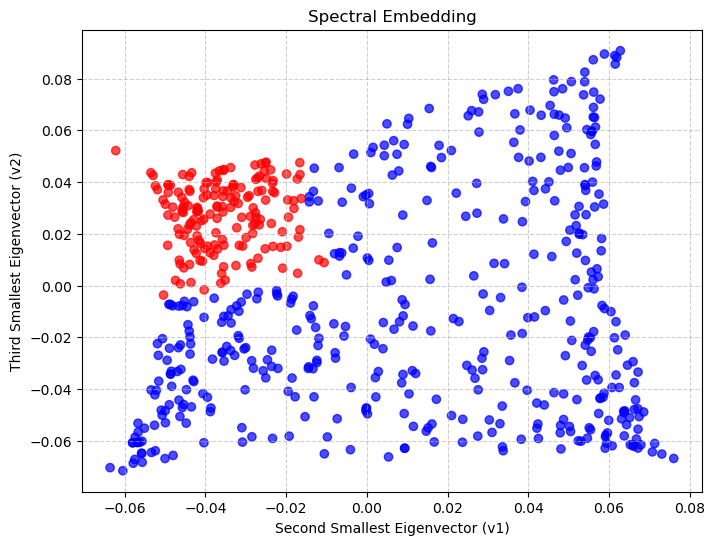
\includegraphics[width=0.8\textwidth]{spectral_embedding.png}
            \caption{Scatter Plot}
        \end{figure}
        
        Red above is where both coordinates have value $<1$. From a heuristic point of view, this should happen around 1/4 of the time, which it looks like it relatively speaking does. All those points that have coordinate $<1$ seem to be in one cluster. This of course makes sense, because if two pairs of points have all coordinates $<$ 1, they are much more likely to be within 1/2 of each other than points than between a point with both coordinates $<$ 1 and another that has some coordinate $>$ 1. So it would be natural that they form a good cluster, which is what the red seems to represent.

        \item Here is the spectral embedding of the graph:
        \begin{figure}[H]
            \centering
            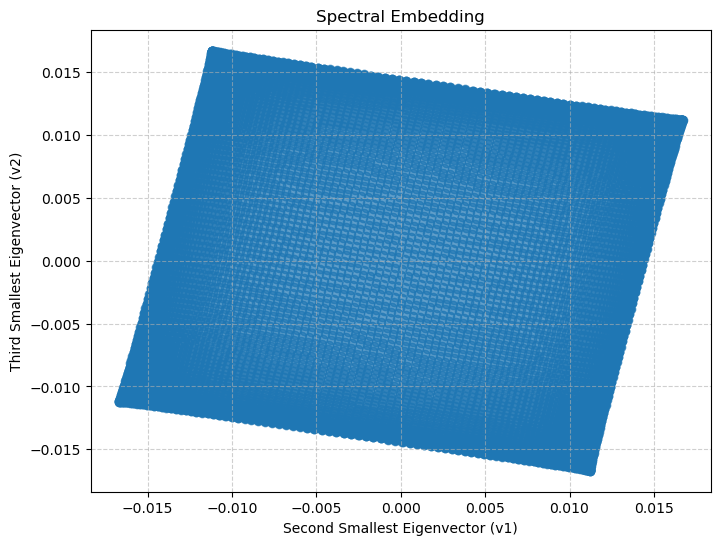
\includegraphics[width=0.8\textwidth]{diamond.png}
            \caption{Spectral Embedding}
        \end{figure}
        Here is the picture with 100 random vertices removed:
        \begin{figure}[H]
            \centering
            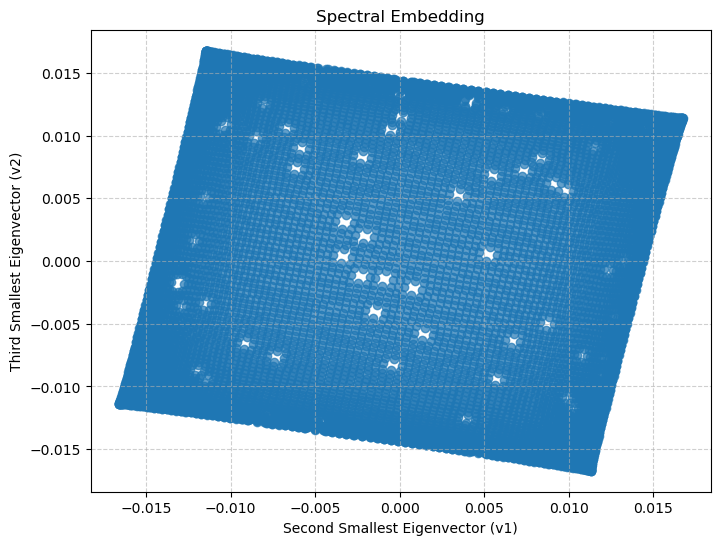
\includegraphics[width=0.8\textwidth]{diamond_holes.png}
            \caption{Spectral Embedding with 100 Random Vertices Removed}
        \end{figure}
        This looks basically the same as the rotated square as before, but with some punctured holes in them. This is representative of how the original graph looks, with the vertices we removed becoming those punctured holes. This picture is shockingly almost the exact same, so I believe this means that the spectral embedding is a very robust algorithm, and a great way to find underlying patterns in graphs, even subject to outside noise.
    \end{enumerate}
    \subsection*{Problem 2: Finding Friends}
    \begin{enumerate}[leftmargin=\labelsep, label=(\alph*)]
        \item Here is a plot of the 12 smallest eigenvalues/vectors of the laplacian of the friendship graph:
        \begin{figure}[H]
            \centering
            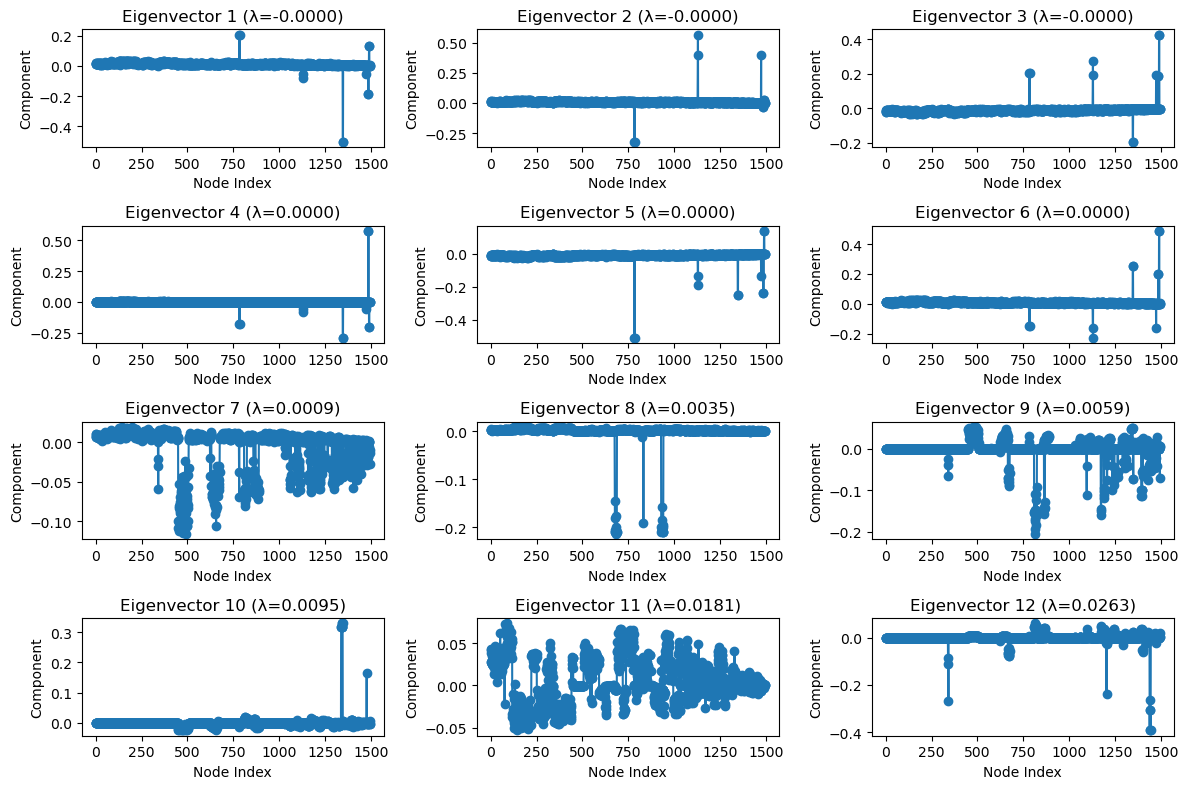
\includegraphics[width=0.8\textwidth]{12_eig.png}
            \caption{Spectral Embedding of Friendship Graph}
        \end{figure}
        \item Recall that the number of components is precisely equal to the number of eigenvalues that are 0 in the Laplacian. In the above picture, eigenvectors 1-6 are 0, so there are 6 connected components. The 7th eigenvalue is not 0. Recall that if $C_1, \ldots, C_k$ are the connected components, the quadratic form becomes:
        \begin{align*}
            x^T L_G x = \sum_{i=1}^k \sum_{u \sim v \in C_i} (x_u-x_v)^2
        \end{align*}
        This is 0 precisely when you assign the same value to every point in a component. So we can simply look at each eigenvector, and make the connected component by putting indices $i$ with the same value for the eigenvectors 1-6 together. For example, in the above picture, the one at around 750 would be in a connected component of its own, since it clearly has a very distinct value from the rest, such as in eigenvector 5. The only way this could contribute 0 to the quadratic form is it if had no neighbors. Let's hope that poor guy makes some friends. It seems like the overwhelming majority of people are in one very large connected component, while there are also a few people who are in connected components of their own. This is quite an interesting result, and I wonder if something could be said about the types of people who stay in their own connected components. Sadly we do not have that data.

        \item The following three sets have conductance far less than 0.1:
        \begin{lstlisting}
the set {2, 4, 6, 8, 9, 11, 13, 17, 18, 21, 24, 25, 33, 36, 41, 43, 54, 55, 60, 66, 67, 71, 76, 83, 84, 86, 87, 89, 92, 95, 109, 111, 112, 115, 117, 121, 122, 125, 129, 133, 136, 137, 138, 140, 141, 144, 148, 149, 150, 151, 152, 155, 158, 160, 161, 163, 165, 170, 172, 173, 175, 176, 177, 180, 184, 187, 190, 192, 193, 198, 201, 202, 203, 204, 205, 206, 207, 208, 217, 223, 226, 228, 231, 233, 235, 243, 247, 248, 249, 251, 252, 255, 256, 263, 264, 272, 276, 279, 280, 284, 288, 289, 293, 294, 295, 297, 306, 307, 314, 318, 321, 323, 325, 328, 332, 335, 339, 340, 344, 348, 352, 354, 355, 356, 360, 367, 371, 372, 386, 388, 389, 390, 396, 398, 399, 403, 404, 407, 412, 415, 416, 418, 420, 424, 425, 426, 432, 436, 438, 439, 440, 445, 446, 449, 450, 451, 453, 456, 457, 461, 462, 466, 467, 469, 471, 477, 478, 480, 485, 488, 495, 498, 499, 502, 503, 504, 506, 507, 510, 512, 513, 515, 518, 519, 520, 521, 522, 527, 530, 534, 538, 540, 542, 545, 546, 547, 551, 552, 554, 558, 560, 563, 572, 573, 579, 581, 584, 588, 590, 591, 593, 594, 595, 596, 597, 598, 599, 606, 608, 611, 612, 615, 616, 630, 631, 635, 639, 642, 643, 650, 651, 657, 661, 663, 674, 677, 679, 680, 685, 686, 694, 699, 705, 706, 707, 709, 711, 715, 718, 719, 720, 723, 724, 731, 739, 743, 748, 749, 759, 760, 761, 763, 764, 765, 769, 773, 774, 778, 781, 782, 789, 793, 796, 798, 799, 801, 802, 804, 811, 812, 814, 816, 818, 819, 820, 822, 824, 825, 827, 831, 833, 836, 837, 841, 842, 850, 851, 853, 854, 858, 865, 866, 867, 869, 871, 872, 873, 876, 877, 881, 882, 884, 887, 889, 891, 893, 896, 897, 899, 905, 906, 912, 920, 922, 924, 926, 931, 932, 933, 935, 937, 940, 941, 942, 944, 945, 952, 955, 957, 962, 963, 968, 972, 974, 976, 979, 980, 981, 983, 995, 996, 999, 1003, 1004, 1008, 1009, 1011, 1013, 1015, 1016, 1017, 1018, 1019, 1023, 1024, 1025, 1028, 1029, 1031, 1032, 1036, 1040, 1041, 1046, 1053, 1054, 1059, 1064, 1069, 1072, 1073, 1080, 1081, 1087, 1089, 1093, 1094, 1095, 1096, 1097, 1098, 1102, 1104, 1105, 1107, 1118, 1121, 1123, 1124, 1125, 1133, 1137, 1138, 1139, 1141, 1144, 1145, 1146, 1148, 1150, 1157, 1158, 1162, 1164, 1166, 1169, 1171, 1172, 1173, 1175, 1179, 1182, 1184, 1185, 1187, 1190, 1191, 1192, 1193, 1195, 1196, 1207, 1211, 1214, 1217, 1218, 1223, 1224, 1227, 1229, 1234, 1235, 1237, 1245, 1247, 1249, 1254, 1260, 1262, 1263, 1270, 1273, 1278, 1281, 1282, 1286, 1288, 1294, 1297, 1299, 1303, 1306, 1307, 1310, 1311, 1315, 1320, 1322, 1323, 1325, 1326, 1333, 1344, 1353, 1361, 1368, 1372, 1373, 1374, 1376, 1379, 1380, 1385, 1388, 1389, 1390, 1392, 1393, 1394, 1395, 1401, 1406, 1412, 1413, 1418, 1422, 1428, 1430, 1436, 1438, 1443, 1444, 1447, 1449, 1458, 1463, 1464, 1466, 1469, 1473, 1478, 1479, 1483, 1484, 1486, 1492, 1493, 1494} has conductance 0.05383895131086142

the set {2, 4, 8, 11, 13, 21, 25, 41, 43, 54, 55, 60, 66, 71, 76, 83, 84, 89, 92, 95, 111, 115, 122, 129, 133, 138, 140, 150, 151, 152, 155, 160, 163, 170, 177, 187, 190, 192, 193, 198, 201, 204, 205, 206, 217, 223, 226, 228, 231, 233, 235, 247, 248, 249, 251, 255, 256, 263, 276, 279, 284, 288, 289, 293, 295, 306, 314, 318, 325, 328, 332, 335, 344, 352, 355, 356, 367, 371, 386, 388, 390, 396, 398, 399, 403, 407, 415, 416, 418, 420, 424, 426, 436, 438, 439, 440, 445, 449, 450, 451, 453, 456, 457, 461, 462, 466, 471, 477, 485, 488, 498, 502, 506, 510, 512, 513, 519, 520, 521, 527, 530, 538, 540, 542, 545, 547, 552, 554, 558, 563, 573, 579, 581, 584, 593, 594, 595, 599, 608, 615, 630, 643, 657, 663, 674, 677, 679, 699, 707, 709, 715, 720, 723, 724, 739, 748, 759, 760, 763, 764, 765, 769, 774, 781, 789, 796, 801, 802, 804, 812, 816, 819, 820, 824, 825, 831, 833, 836, 837, 841, 842, 851, 858, 866, 873, 876, 889, 891, 896, 899, 912, 920, 924, 926, 931, 935, 937, 941, 944, 945, 952, 955, 957, 968, 972, 979, 980, 981, 983, 995, 996, 1004, 1008, 1011, 1015, 1016, 1017, 1018, 1019, 1025, 1028, 1029, 1032, 1036, 1040, 1053, 1059, 1064, 1072, 1081, 1095, 1096, 1097, 1102, 1104, 1105, 1107, 1118, 1121, 1124, 1125, 1133, 1137, 1139, 1141, 1144, 1145, 1148, 1150, 1166, 1171, 1173, 1175, 1182, 1185, 1187, 1191, 1192, 1193, 1195, 1196, 1218, 1223, 1227, 1234, 1235, 1237, 1247, 1254, 1260, 1262, 1263, 1270, 1273, 1281, 1282, 1294, 1299, 1310, 1315, 1320, 1325, 1326, 1344, 1368, 1372, 1373, 1380, 1385, 1390, 1392, 1393, 1394, 1395, 1406, 1412, 1413, 1422, 1436, 1438, 1443, 1444, 1449, 1463, 1464, 1466, 1469, 1473, 1479, 1484, 1486, 1493, 1494} has conductance 0.09870598856455011

the set {2, 4, 8, 11, 13, 17, 21, 25, 41, 43, 54, 55, 60, 66, 67, 71, 76, 83, 84, 89, 92, 95, 111, 115, 122, 129, 133, 138, 140, 150, 151, 152, 155, 158, 160, 163, 170, 177, 187, 190, 192, 193, 198, 201, 203, 204, 205, 206, 217, 223, 226, 228, 231, 233, 235, 247, 248, 249, 251, 255, 256, 263, 276, 279, 284, 288, 289, 293, 295, 306, 314, 318, 325, 328, 332, 335, 344, 348, 352, 355, 356, 367, 371, 386, 388, 390, 396, 398, 399, 403, 407, 415, 416, 418, 420, 424, 426, 436, 438, 439, 440, 445, 449, 450, 451, 453, 456, 457, 461, 462, 466, 471, 477, 485, 488, 498, 502, 503, 506, 510, 512, 513, 519, 520, 521, 527, 530, 538, 540, 542, 545, 547, 551, 552, 554, 558, 563, 573, 579, 581, 584, 593, 594, 595, 599, 608, 611, 615, 630, 643, 657, 663, 674, 677, 679, 699, 707, 709, 715, 720, 723, 724, 739, 748, 759, 760, 763, 764, 765, 769, 774, 781, 789, 796, 801, 802, 804, 812, 816, 819, 820, 824, 825, 827, 831, 833, 836, 837, 841, 842, 851, 858, 866, 873, 876, 877, 889, 891, 896, 897, 899, 912, 920, 924, 926, 931, 935, 937, 941, 944, 945, 952, 955, 957, 968, 972, 974, 979, 980, 981, 983, 995, 996, 1004, 1008, 1011, 1015, 1016, 1017, 1018, 1019, 1025, 1028, 1029, 1032, 1036, 1040, 1053, 1059, 1064, 1072, 1081, 1095, 1096, 1097, 1102, 1104, 1105, 1107, 1118, 1121, 1124, 1125, 1133, 1137, 1139, 1141, 1144, 1145, 1148, 1150, 1166, 1171, 1173, 1175, 1182, 1185, 1187, 1191, 1192, 1193, 1195, 1196, 1217, 1218, 1223, 1227, 1234, 1235, 1237, 1247, 1254, 1260, 1262, 1263, 1270, 1273, 1281, 1282, 1294, 1299, 1307, 1310, 1315, 1320, 1325, 1326, 1333, 1344, 1368, 1372, 1373, 1380, 1385, 1388, 1390, 1392, 1393, 1394, 1395, 1406, 1412, 1413, 1422, 1436, 1438, 1443, 1444, 1449, 1463, 1464, 1466, 1469, 1473, 1479, 1484, 1486, 1493, 1494} has conductance 0.08027691854470467
        \end{lstlisting}
        I used the algorithm that we used in class to prove Cheeger's inequality to find these. I used the 7th smallest eigenvector of the laplacian graph, since above we had 6 connected components, so to find a good cluster I needed to use the first eigenvector that did not have a 0 eigenvalue. (You could theoretically just use a connected component, but I believe the sum of all the non-huge connected components has less than 200 people, so this doesn't work). I then sorted the indices by the value of the eigenvector, and then tried all possible thresholds that yield more than 200 people for both $S$ and $V \setminus S$ to find a good conductance set. I outputted all the ones that were less than 0.1 and then proceeded to just pick three random ones.

        \item I found the conductance for a random set of 200 nodes 10 times, and got the following output:
        \begin{lstlisting}
Conductance of random subset: 0.8478465891229173
Conductance of random subset: 0.8873684210526316
Conductance of random subset: 0.8723350573987637
Conductance of random subset: 0.8645857241221023
Conductance of random subset: 0.8687306501547988
Conductance of random subset: 0.862488306828812
Conductance of random subset: 0.8714285714285714
Conductance of random subset: 0.8704537582265327
Conductance of random subset: 0.8664112999760594
Conductance of random subset: 0.8585929296464824
        \end{lstlisting}
        These are horrible! The sets we found before must be extremely tight-knit compared to a random set of people. Like a very tight friendgroup.
    \end{enumerate}
\end{document}